\chapter{Analisi prerequisiti e possibili soluzioni}
\label{sec:analisi_ricerca}

Una volta esaminata l'implementazione attuale e identificati i suoi principali
problemi nel capitolo precedente, è stato deciso di utilizzare un approccio DRY.
L'acronimo DRY, Don't Repeat Yourself, si riferisce al principio in Computer
Science in cui "Ogni conoscenza deve avere una rappresentazione unica, univoca e
autorevole all’interno di un sistema" descritto in \texttt{The Pragmatic
Programmer}\cite{thomas2019pragmatic}. In questo caso ne viene esteso il
significato per riferirsi all'utilizzo di framework esterni testati e che hanno
dimostrato di funzionare.

\section{Prerequisiti}
\label{sec:prerequisiti}

Viene proposta ora un'analisi esaustiva dei prerequisiti da considerare e valutare
durante il processo di ricerca \ref{sec:candidates} e scelta \ref{sec:airflow} del
framework che verrà usato per sostituire l'attuale implementazione. Si
individuano i prerequisiti fondamentali riportati di seguito.

\subsection{Utilizzo efficiente delle risorse}
\label{sub:resource_usage}

Primo prerequisito fondamentale è la possibilità di sfruttare completamente le risorse
a disposizione. Questo significa che bisognerà inizialmente favorire la
scalabilità verticale del sistema, in questo modo è possibile partire da un sistema
più semplice che verrà esteso in seguito. Scalare verticalmente comporta creare
una macchina unica più potente e risparmiare nel complesso risorse, in quanto l'overhead
del sistema operativo è presente soltanto una volta e un core può effettivamente
eseguire più task alla volta sfruttando il multithreading.

\subsection{Definizione dipendenze tramite DAG}
\label{sub:deps_definition}

Come visto nella sezione \ref{sub:robots}, vengono definite delle dipendenze tra
fasi. Uno dei prerequisiti fondamentali è la possibilità di definire in modo
esplicito grafi di dipendenze, non dovendo quindi pensare per ogni fase quali devono
essere quelle che la precedono o la seguono. Sarebbe ideale un'implementazione
analoga a quella riportata nel codice \ref{lst:dag-example} e renderizzata in
figura \ref{fig:dag-example}.

\begin{figure}[htbp]
  \centering
  \begin{minipage}{0.45\textwidth}
    \centering
    \lstinputlisting[language=Python, caption=Esempio di definizione di DAG in Airflow,
    label=lst:dag-example ]{listings/dag-example.py}
  \end{minipage}
  \hfill
  \begin{minipage}{0.45\textwidth}
    \centering
    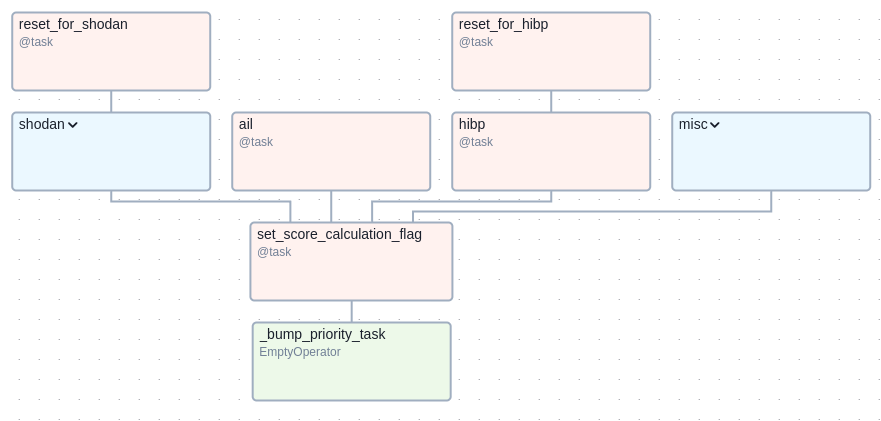
\includegraphics[width=\textwidth]{images/dag-example.png}
    \caption{Esempio di renderizzazione del DAG}
    \label{fig:dag-example}
  \end{minipage}
\end{figure}

\subsection{Compatibilità con Python}
\label{sub:python_compatibility}

Il linguaggio di programmazione principale, in cui è scritta la parte di collezione
e serializzazione dei dati, è Python. Questo significa che gran parte delle fasi
eseguite dalle macchine Robot possono essere utilizzate nella nuova implementazione
senza cambiamenti radicali. Data la natura della maggior parte delle task, che svolgendo
ricerche OSINT, vengono eseguite molte richieste di rete. Ciò significa che, per
la maggior parte del tempo, il processo resta in attesa di una risposta da un server
remoto (I/O intensive) e non esegue operazioni computazionalmente pesanti (CPU
intensive). Per questo motivo utilizzare un linguaggio di programmazione più
performante non aumenterebbe molto le prestazioni e aggiungerebbe soltanto
complessità nel tradurre le implementazioni attuali e gestire codice in un
linguaggio poco conosciuto dal team.

Un'altra caratteristica fondamentale e correlata è la possibilità di definire le
task in modo programmatico, in modo da appunto riutilizzare il codice già presente
e funzionante.

\subsection{Scalabilità orizzontale}
\label{sub:scalable}

Espandendo quanto descritto al requisito \ref{sub:resource_usage}, potrebbe presentarsi
la necessità di scalare e utilizzare più risorse di quelle messe a disposizione dall'infrastruttura
sottostante. Questo problema può essere risolto utilizzando un approccio di
scalabilità orizzontale. Il framework selezionato deve quindi offrire la possibilità
di funzionare su cluster in modo relativamente semplice e veloce, idealmente
utilizzando soluzioni ben conosciute quali Kubernetes\cite{kubernetes}.

\subsection{Open source, Manutenzione e Documentazione}
\label{sub:open_source}

Prima di valutare strumenti offerti da altre aziende come prodotti a pagamento, è
opportuno valutare la presenza di eventuali strumenti Open source o disponibili gratuitamente.
In ambito Open source bisogna prestare particolare attenzione a tre aspetti
chiave: la manutenzione, ovvero quanto attivo è il progetto e quanto velocemente
vengono risolti bug e implementate nuove funzionalità; il supporto, ovvero
quanto è attiva la comunità attorno al progetto per chiedere aiuto in caso di
problemi o difficoltà nell'utilizzo del framework; completezza e chiarezza della
documentazione, fondamentale per utilizzare in modo efficiente tutte le
funzionalità del software in questione.

\subsection{Isolabilità}
\label{sub:isolation}

Alcune fasi implementate all'interno di SATAYO necessitano di un ambiente isolato
per essere eseguito correttamente. Esempio pratico di questo requisito potrebbe
essere l'utilizzo di una VPN, che forza tutto il traffico del sistema ad uscire attraverso
di essa; questo non permetterebbe a determinate altre fasi di comunicare
correttamente con il server remoto a cui si appoggiano. Analogamente se una determinata
fase utilizza un software Open source di dubbia sicurezza, o con dipendenze
molto vecchie che andrebbero in conflitto con il resto del sistema, è opportuno che
vengano eseguite le fasi all'interno di sandbox che ne limitino le capacità.

\subsection{Monitorabilità}
\label{sub:monitorable}

Ultimo requisito fondamentale è la possibilità di poter monitorare a fondo lo
stato del sistema, ma soprattutto lo stato delle singole fasi che sono in esecuzione.
Più specificatamente è necessario avere una visione molto dettagliata della
parte di schedulazione implementata dal framework, il quale deve mettere a disposizione
metriche collezionabili da sistemi di monitoraggio quali Neteye\cite{neteye} o
Prometheus\footnote{\url{https://prometheus.io/}}.

Per quanto riguarda il collezionamento dei log di esecuzione delle fasi, deve
esserci un metodo standardizzato per produrli in modo tale che possano essere
collezionati da sistemi di collezionamento e indicizzazione come Elasticsearch\footnote{\url{https://www.elastic.co/elasticsearch}}.

\section{Soluzioni candidate}
\label{sec:candidates}

Durante l'attività di ricerca sono state individuate più soluzioni e framework
che rispettavano alcuni o tutti i requisiti definiti nella sezione precedente. Di
seguito sono riportate le caratteristiche dei candidati più interessanti che sono
stati valutati per la scelta finale, la tabella \ref{table:requisites} riporta
una visualizzazione di tutti i requisiti per ogni framework.

\begin{itemize}
  \item \textbf{multithreading nativo di Python:} prima possibile soluzione, è stata
    immediatamente scartata in quanto rispetta solo il requisito \ref{sub:resource_usage}
    (e naturalmente \ref{sub:python_compatibility}). Nonostante ciò è risultata
    molto utile per individuare correttamente il requisito \ref{sub:open_source};

  \item \textbf{Celery\footnote{\url{https://docs.celeryq.dev/en/stable/}}:} è
    il primo framework effettivo analizzato come possibile opzione, dalla documentazione
    ufficiale "Celery è un sistema distribuito semplice, flessibile e affidabile
    per elaborare grandi quantità di messaggi, fornendo al tempo stesso alle
    operazioni gli strumenti necessari per mantenere tale sistema". Data questa
    definizione Celery sembra un ottimo candidato, soddisfa pienamente i requisiti:
    \ref{sub:resource_usage} in quanto un nodo worker può sfruttare al meglio le
    risorse eseguendo più fasi in diversi sottoprocessi; \ref{sub:python_compatibility}
    perché scritto interamente in Python e completamente compatibile con esso;
    \ref{sub:open_source} in quanto il progetto è molto grande e mantenuto. Contrariamente
    in Celery non esiste un modo conciso di definire dipendenze tramite DAG,
    \ref{sub:deps_definition}. Esiste la possibilità di scalare orizzontalmente come
    richiesto da \ref{sub:scalable} aggiungendo nodi worker al sistema, bisogna
    però gestirli manualmente e non può essere delegato a piattaforme pre
    esistenti quali Kubernetes. Infine rispetta parzialmente anche il requisito \ref{sub:isolation}
    in quanto nonostante non ci sia un metodo nativo di implementarlo, si
    possono creare più worker in ambienti dedicati diversi, ed eseguire determinate
    task con requisiti particolari in quest'ultimi.

  \item \textbf{Luigi\footnote{\url{https://github.com/spotify/luigi}}:} è un
    pacchetto Python che serve per "costruire pipeline complesse di lavori batch"
    come riportato nella documentazione del progetto. Purtroppo per questo caso d'uso
    Luigi risulta essere troppo semplice e limitante, in quanto come Celery non
    supporta la definizione esplicita di DAG \ref{sub:deps_definition}. Inoltre non
    permette la scalabilità orizzontale \ref{sub:scalable}, né l'isolabilità
    \ref{sub:isolation}; ha una documentazione alquanto limitata e non mette a disposizione
    molte metriche per il monitoraggio.

  \item \textbf{Apache Airflow\cite{airflow}:} come descritto nella pagina
    principale del progetto, "Airflow è una piattaforma creata dalla community
    per progettare, pianificare e monitorare in modo programmatico i flussi di lavoro",
    rispetta tutti i requisiti descritti nella sezione \ref{sec:prerequisiti} ed
    è stato scelto come core della nuova implementazione. Verrà descritto più
    nel dettaglio come questo framework ha soddisfatto i requisiti imposti nella
    sezione \ref{sec:airflow}.
\end{itemize}

\begin{table}[htbp]
  \begin{center}
    \renewcommand{\arraystretch}{1.5}
    \begin{tabular}{|>{\centering\arraybackslash}m{6cm}|>{\centering\arraybackslash}m{3cm}|c|c|c|}
      \hline
      \textbf{Requisito}                 & \textbf{Multithreading nativo} & \textbf{Luigi} & \textbf{Celery} & \textbf{Apache Airflow} \\
      \hline
      \nameref{sub:resource_usage}       & \cmark                         & \cmark         & \cmark          & \cmark                  \\
      \hline
      \nameref{sub:deps_definition}      & \xmark                         & \xmark         & \xmark          & \cmark                  \\
      \hline
      \nameref{sub:python_compatibility} & \cmark                         & \cmark         & \cmark          & \cmark                  \\
      \hline
      \nameref{sub:scalable}             & \xmark                         & \xmark         & \imark          & \cmark                  \\
      \hline
      \nameref{sub:open_source}          & \imark                         & \imark         & \cmark          & \cmark                  \\
      \hline
      \nameref{sub:isolation}            & \xmark                         & \xmark         & \imark          & \cmark                  \\
      \hline
      \nameref{sub:monitorable}          & \xmark                         & \imark         & \cmark          & \cmark                  \\
      \hline
    \end{tabular}
  \end{center}
  \caption{Requisiti soddisfatti (\cmark), non pienamente soddisfatti (\imark) e
  non soddisfatti (\xmark) da ciascun framework}
  \label{table:requisites}
\end{table}

\section{Apache Airflow}
\label{sec:airflow}

Come precedentemente accennato, Apache Airflow risulta essere il candidato
ideale per modernizzare l'infrastruttura di SATAYO. Più dettagliatamente Airflow
soddisfa tutti i requisiti elencati nella sezione \ref{sec:prerequisiti} nel seguente
modo:

\begin{itemize}
  \item \textbf{\nameref{sub:resource_usage}:} le task all'interno di Airflow
    vengono eseguite tramite un Executor. Gli Executor di Airflow sono progettati
    in modo tale da rispettare un'interfaccia comune ed essere intercambiabili.
    In questo caso particolare, viene utilizzato il \texttt{CeleryExecutor} che
    utilizza lo stesso Celery come backend per l'esecuzione delle task, permettendo
    un utilizzo efficiente delle risorse della macchina tramite multithreading;

  \item \textbf{\nameref{sub:deps_definition}:} come è possibile vedere nel
    codice di esempio \ref{lst:dag-example}, Airflow, in determinati contesti, modifica
    la funzionalità degli operatori di bitshift (\texttt{<<} e \texttt{>>}) e delle
    liste (\texttt{[...]}) permettendo quindi una scrittura concisa ed esplicita
    delle dipendenze tra le task. Prendendo come esempio la seguente espressione,
    si può intuitivamente dedurre che vengano eseguite nell'ordine \textit{first\_task},
    \textit{second\_task} e poi simultaneamente \textit{third\_task} e \textit{fourth\_task};

    \begin{lstlisting}[language=Python]
first_task >> second_task >> [third_task, fourth_task]
\end{lstlisting}

  \item \textbf{\nameref{sub:python_compatibility}:} Airflow è completamente
    scritto in Python, ciò implica che anche le task siano definite da funzioni Python
    e quindi implementare su Airflow le fasi già presenti su SATAYO risulta triviale.
    Airflow risulta essere molto flessibile riguardo a come è implementata la
    funzione che viene eseguita, permettendo di utilizzare implementazioni in svariati
    linguaggi di programmazione in modo nativo tramite diversi Operator. Un
    Operator non è altro che una task che svolge delle azioni predefinite, utilizzando
    degli argomenti dati;

  \item \textbf{\nameref{sub:scalable}:} utilizzando Celery come backend, Airflow
    riporta gli stessi vantaggi e svantaggi, in breve è possibile scalare
    orizzontalmente con Celery, ma è molto dispendioso a livello di tempo.
    Fortunatamente Airflow è nativamente compatibile con Kubernetes e offre come
    Executor alternativo il KubernetesExecutor che esegue ogni task su un Pod
    dedicato, lasciando quindi la gestione delle risorse al cluster sottostante.
    Grazie a Kubernetes, per aggiungere nodi al cluster, è sufficiente creare
    una nuova macchina, installare Kubernetes e adottarla all'interno del cluster
    con pochi comandi;

  \item \textbf{\nameref{sub:open_source}:} lo sviluppo del progetto Apache
    Airflow è sostenuto dalla \textit{Apache Software Foundation}\footnote{\url{https://apache.org/index.html}}
    che ad oggi conta più di 320 progetti Open source. Inoltre, il progetto
    Airflow è molto attivo su GitHub, con circa 100 commit alla settimana nell'ultimo
    periodo e oltre \num{35000} stelle sulla repository. In aggiunta è presente una
    community molto grande sulla piattaforma Slack, e una documentazione molto
    vasta, completa e dettagliata in cui è possibile trovare tutto ciò che riguarda
    l'utilizzo del progetto;

  \item \textbf{\nameref{sub:isolation}:} come accennato precedentemente, Airflow
    mette a disposizione diversi Operator, i quali permettono di eseguire task
    predeterminate o in diversi ambienti. Tra questi sono riportati i più interessanti
    nell'ambito di isolabilità dell'esecuzione: il \texttt{PythonVirtualenvOperator}
    permette di eseguire codice Python all'interno di un Virtualenvironment,
    consentendo l'utilizzo di dipendenze diverse o che potrebbero creare
    conflitti; il \texttt{DockerOperator} permette di creare un container Docker
    da un'immagine specificata, e di eseguire all'interno di esso il codice o programma
    impostato, isolando di conseguenza l'intera esecuzione del programma dal
    resto del sistema. Infine, nel caso in cui venga usato il \texttt{KubernetesExecutor},
    l'esecuzione di ciascuna task è contenuta all'interno di un Pod che viene
    creato appositamente e distrutto successivamente alla terminazione della
    funzione.

  \item \textbf{\nameref{sub:monitorable}:} concludendo, per quanto riguarda il monitoraggio
    dell'intero sistema, Airflow mette a disposizione molte metriche relative
    all'esecuzione delle task e allo stato del sistema stesso. Le metriche in questione
    possono essere esportate da Airflow utilizzando due formati standard:
    \texttt{StatsD} e \texttt{OpenTelemetry}. Infine i messaggi di log delle singole
    task risultano molto configurabili ed è possibile impostare il modulo in modo
    tale che questi vengano salvati sul filesystem locale, oppure esportati
    direttamente verso servizi di terze parti.
\end{itemize}